% THIS IS SIGPROC-SP.TEX - VERSION 3.1
% WORKS WITH V3.2SP OF ACM_PROC_ARTICLE-SP.CLS
% APRIL 2009
%
% It is an example file showing how to use the 'acm_proc_article-sp.cls' V3.2SP
% LaTeX2e document class file for Conference Proceedings submissions.
% ----------------------------------------------------------------------------------------------------------------
% This .tex file (and associated .cls V3.2SP) *DOES NOT* produce:
%       1) The Permission Statement
%       2) The Conference (location) Info information
%       3) The Copyright Line with ACM data
%       4) Page numbering
% ---------------------------------------------------------------------------------------------------------------
% It is an example which *does* use the .bib file (from which the .bbl file
% is produced).
% REMEMBER HOWEVER: After having produced the .bbl file,
% and prior to final submission,
% you need to 'insert'  your .bbl file into your source .tex file so as to provide
% ONE 'self-contained' source file.
%
% Questions regarding SIGS should be sent to
% Adrienne Griscti ---> griscti@acm.org
%
% Questions/suggestions regarding the guidelines, .tex and .cls files, etc. to
% Gerald Murray ---> murray@hq.acm.org
%
% For tracking purposes - this is V3.1SP - APRIL 2009

\documentclass{acm_proc_article-sp}

\newcommand{\upcite}[1]{\textsuperscript{\textsuperscript{\cite{#1}}}}

\begin{document}

\title{Attack On Drones}
%
% You need the command \numberofauthors to handle the 'placement
% and alignment' of the authors beneath the title.
%
% For aesthetic reasons, we recommend 'three authors at a time'
% i.e. three 'name/affiliation blocks' be placed beneath the title.
%
% NOTE: You are NOT restricted in how many 'rows' of
% "name/affiliations" may appear. We just ask that you restrict
% the number of 'columns' to three.
%
% Because of the available 'opening page real-estate'
% we ask you to refrain from putting more than six authors
% (two rows with three columns) beneath the article title.
% More than six makes the first-page appear very cluttered indeed.
%
% Use the \alignauthor commands to handle the names
% and affiliations for an 'aesthetic maximum' of six authors.
% Add names, affiliations, addresses for
% the seventh etc. author(s) as the argument for the
% \additionalauthors command.
% These 'additional authors' will be output/set for you
% without further effort on your part as the last section in
% the body of your article BEFORE References or any Appendices.

\numberofauthors{5} %  in this sample file, there are a *total*
% of EIGHT authors. SIX appear on the 'first-page' (for formatting
% reasons) and the remaining two appear in the \additionalauthors section.
%
\author{
% You can go ahead and credit any number of authors here,
% e.g. one 'row of three' or two rows (consisting of one row of three
% and a second row of one, two or three).
%
% The command \alignauthor (no curly braces needed) should
% precede each author name, affiliation/snail-mail address and
% e-mail address. Additionally, tag each line of
% affiliation/address with \affaddr, and tag the
% e-mail address with \email.
%
% 1st. author
\alignauthor
Yan Songyang\\
       \affaddr{School of Software Engneering}\\
       \affaddr{Xi'an Jiaotong University}\\
       \email{lapalacayim@gmail.com}
% 2nd. author
\alignauthor
Li Siyu\\
       \affaddr{College of Cybersecurity}\\
       \affaddr{Sichuan University}\\
       \email{sy\_lee\_real@icloud.com}
% 3rd. author
\alignauthor Wan Ziyi\\
       \affaddr{College of Cybersecurity}\\
       \affaddr{Sichuan University}\\
       \email{scuderrickwan@gmail.com}
\and  % use '\and' if you need 'another row' of author names
% 4th. author
\alignauthor Ye Junyan\\
       \affaddr{School of Information and Software Engineering}\\
       \affaddr{University of Electronic Science and Technology}\\
       \email{2239308357@qq.com}
% 5th. author
\alignauthor Li Hanxing\\
       \affaddr{School of Cyber Science and Engineering}\\
       \affaddr{Wuhan University}\\
       \email{t0918555@u.nus.edu}
}
% There's nothing stopping you putting the seventh, eighth, etc.
% author on the opening page (as the 'third row') but we ask,
% for aesthetic reasons that you place these 'additional authors'
% in the \additional authors block, viz.
% Just remember to make sure that the TOTAL number of authors
% is the number that will appear on the first page PLUS the
% number that will appear in the \additionalauthors section.

\maketitle
\begin{abstract}
In this article we investigate the security problems of the Parrot AR.Drone 2.0 and Hubsan H107 quadcopters. We will set focus mainly on obvious security vulnerabilities in the Wi-Fi and 2.4GHz radio connection. We will show how to eavesdrop video streams of the AR.Drones and take over it's control using Man-In-The-Middle attack. We will illustrate the approach of radio replay attack on the Hubsan H107. Besides the realization of attacks, we put forward some suggestions on how the drones could be secured from unauthorized access.
\end{abstract}

% A category with the (minimum) three required fields
\category{H.4}{Input/Output and Data Communications}{Data Communication Devices}


%\terms{Theory}

\keywords{Drone, Remote Control, Man-In-The-Middle, Replay Attack} % NOT required for Proceedings

\section{Introduction}

 The drone, also known as the unmanned aerial vehicle(UAV), is the Aircraft without  any human pilot controlling inside. Drones are widely used in many fields, including military, industry, agriculture, photography and so on. We can simply divide them into civilian and military. 
 
 
 The civilian drones, which we are focusing on, are applied to countless aspects of our lives.  Farmers use drones to spray pesticides and monitor crop's growth. E-commerce companies such as Amazon use drones to deliver express. Photographers use drones to create from a special perspective. And also people, just like us, using drones just for fun. All in all, the use of drones has penetrated into many aspect of our lives.
 
 
  Quadcopter, one of the most common types of civilian drones, using Wi-Fi connection or 2.4GHz radio as its way of communication, generally. Some professional drone companies such as DJI may have their own private communication protocols and they are beyond our research.
  
  
 Within Wi-Fi connection, a drone is WLAN AP(Access Point) itself. If the user wants to control the drone, he needs to connect his smartphone(or other smart devices) with control application to the WLAN created by the drone. And there may be steps to authenticate during the connection establishment process. Then user's smartphone could issue instructions to the drone and receive real-time image transmission from drone, after getting the Wi-Fi connection to the drone.
 
 
 And the other way of communication is using 2.4GHz radio. This is a much simpler communication mechanism, which means it has a lower cost and usually used on low-end drones. 2.4GHz radio technique is widely used in lots of remote controls, and remote control used in toys including drones is the one of the application scenarios. The remote control sending instructions via an agreed frequency in 2.4GHz ISM, and the drone receive these instructions. The massage transmit via 2.4GHz radio broadcasts to anyone that can receive it, which means there isn't any connection between remote control and the drone. Not to mention identity verification. So this is a primitive way of control, which is easy to attack.

\section{Attack on the AR.Drone 2.0}

In this section, we investigate the security vulnerabilities of AR.Drone 2.0 and conduct two attacks on the drone.

\subsection{Technical Specification}
The specifications of the AR.Drone 2.0 are as follows:

\begin{itemize}
  \item Battery: 1500 mAH battery providing up to 36 minutes of flight time.
  \item Weight: With Indoor frame: 420 gram, With outdoor frame: 380 gram.
  \item Radio: Unencrypted 2.4 GHz Wi-Fi smartphone controlled.
  \item A GPS module is available as an add on to the USB port of the drone to fly.
  \item OS: BusyBox V1.14.0,  a Linux operating system based on the kernel version 2.6.27.44.
pre-planned routes.
\end{itemize}

Users can use iOS and Android devices to control the drone via the official application AR.FreeFlight. Figure ~\ref{iPad} shows the controller interface running on iPad. 

\begin{figure}
\centering
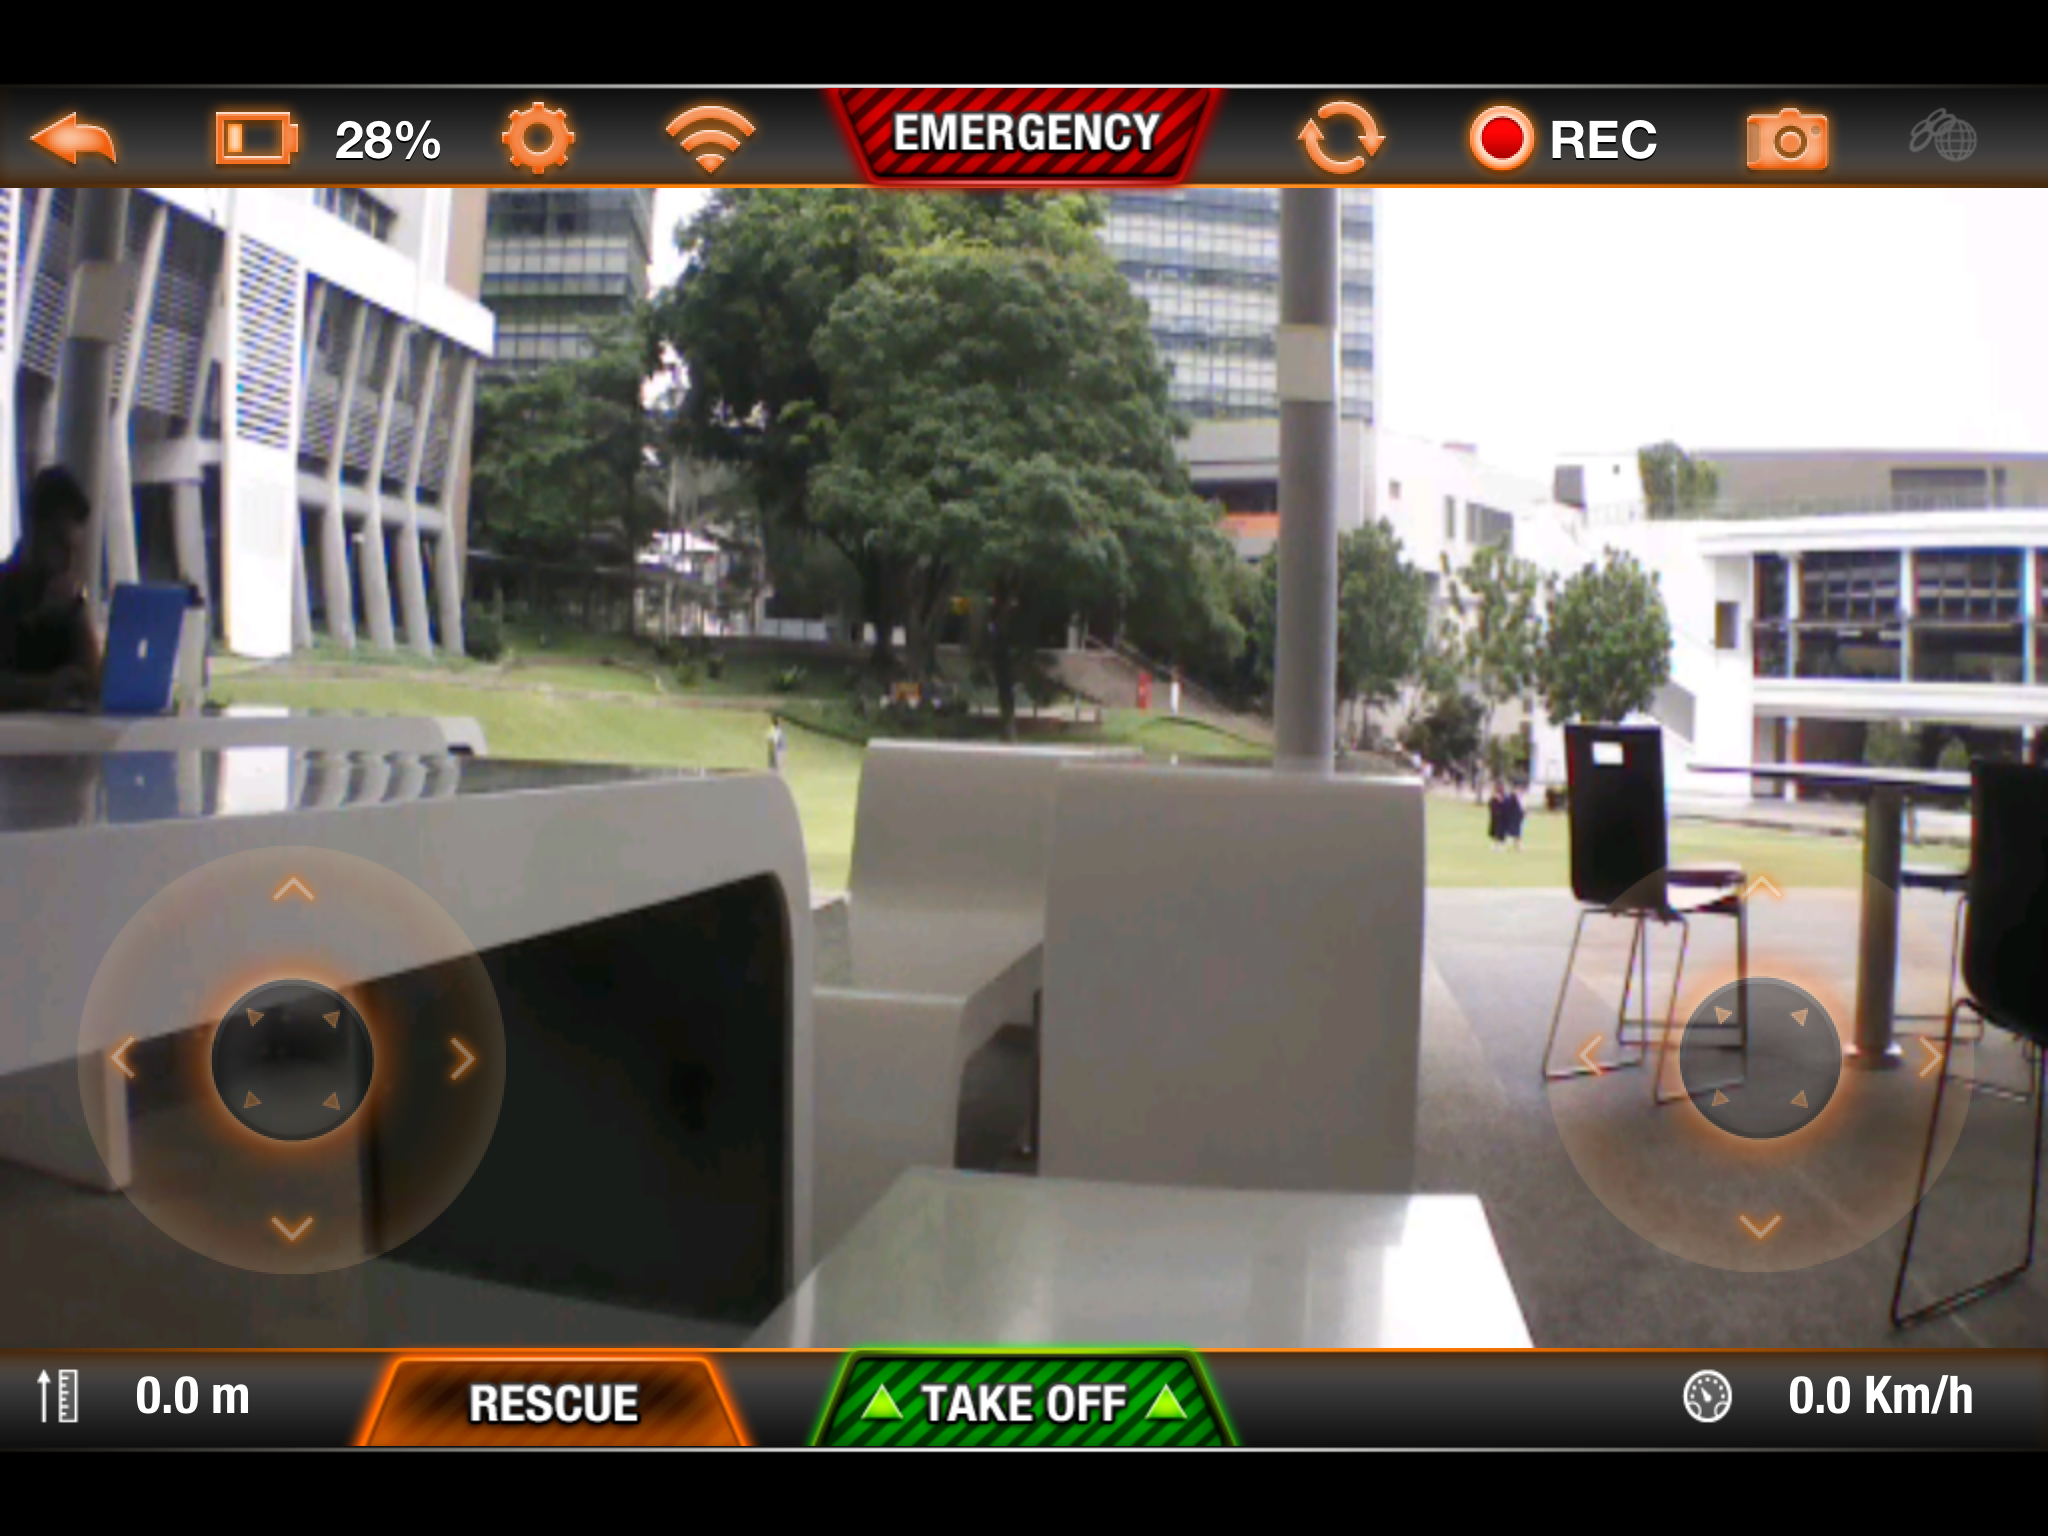
\epsfig{file=figures/iPad.PNG, height=1.2in, width=1.8in}
\caption{Parrot AR.FreeFlight control interface}
\label{iPad}
\end{figure}

After scanning the open ports running on the drone, we found that it has open Telnet port with root access giving full access to the drone system. It is such a catastrophic vulnerability that the drone can be crashed by killing the jobs running on the Linux system. The exploitation of this vulnerability is stated in ~\cite{ana:attack}.

\subsection{Video Signal Interception}

According to AR.Drone Developer Guide\upcite{dev:guide}, AR.Drone 2.0 video stream is transmitted on TCP socket 5555. AR.Drone 2.0 will start sending frame immediately when a client connects to the socket. 

For drones like JJRC-H37 produced by JIANJIAN TECHNOLOGY, they broadcast video signal to every client. Hence every device that connected to the drone can watch the video stream simultaneously. While AR.Drone 2.0 only sends video stream to the controller. To eavesdrop the video stream sent by AR.Drone 2.0, attacker can do as follows:

\begin{enumerate}
  \item Connection to the drone,
  \item Determination of the IP address of the control device,
  \item Using arp spoofing to intercept data,
  \item Decode video stream.
\end{enumerate}

In this project, we use Ettercap\upcite{ettercap} to conduct Man-In-The-Middle attack using arp poisoning. The drone's ip address is 192.168.1.1 and the controller's ip address is 192.168.1.2. The configuration of Ettercap is shown as figure~\ref{ettercap}.

\begin{figure}
\centering
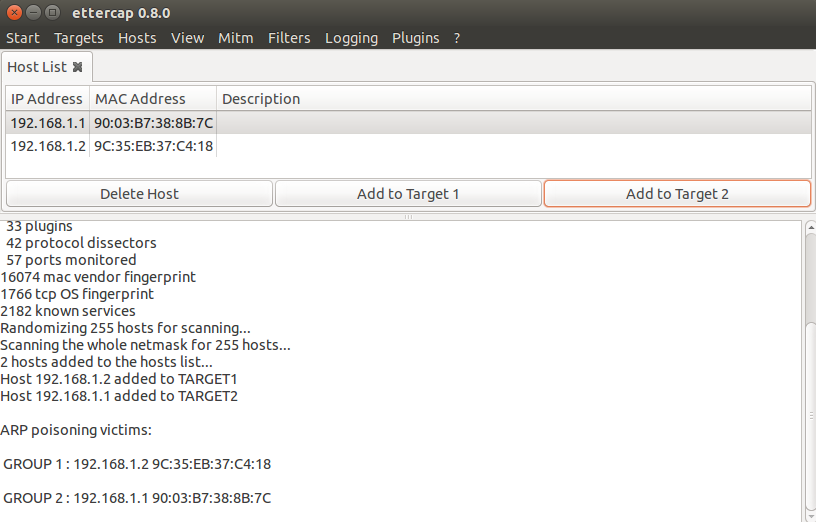
\epsfig{file=figures/ettercap.png, height=1.2in, width=1.8in}
\caption{Ettercap Configuration}
\label{ettercap}
\end{figure}


AR.Drone SDK 2 \upcite{sdk} provides us a tool called ardrone\_navigation to decode video stream. It receives data stream from drone. The video module inside will decode the stream and show it in a seperated window. Figure~\ref{navigation} shows the user interface of ardrone\_navigation.

\begin{figure}
\centering
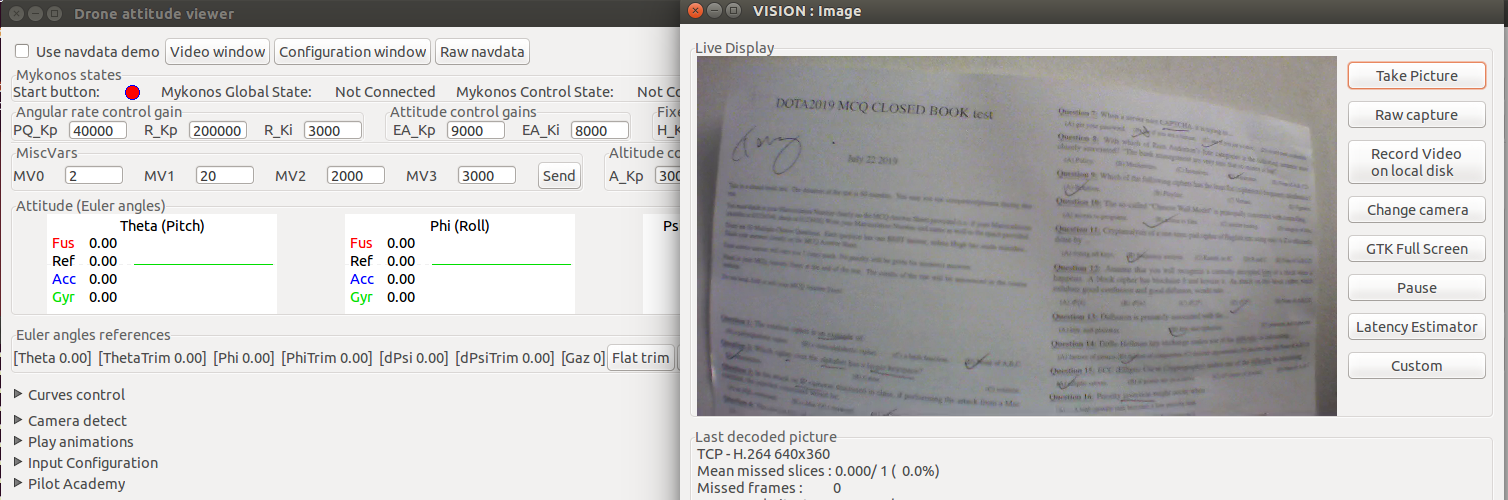
\epsfig{file=figures/navigation.png, height=0.8in, width=2.4in}
\caption{GUI of ardrone\_navigation}
\label{navigation}
\end{figure}


\subsection{Highjack Attack}

\subsubsection{AT Commands}
 The controller uses port 5556 to send commands in a UDP packet to port 5556 of the drone\upcite{dev:guide}. These commands are called AT commands. Because of the instability of UDP connection, the communication protocol allocates ascending sequence number to different commands. This prevents older commands with lower sequence numbers incoming later (due to transmission errors) from executing\upcite{hack:secure}. This protocol provides an attack method. Attacker can conduct a man-in-the-middle attack with a sequence number which is always higher than the one being sent from the legitimate user.

An AT command begins with the fixed string "AT*", followed by either REF, PCMD or CONFIG. REF commands are single commands such as land or takeoff. PCMD commands are used for flight control. CONFIG commands are used for sending new configuration. To take over a drone, using REF commands is enough. The format command of REF command is 
\begin{equation}
  AT*REF=<sequence>,<UI>.
\end{equation}


Different REF commands are listed in table ~\ref{refcom}.

\begin{table}
\centering
\caption{REF commands}
\label{refcom}
\begin{tabular}{@{}ll@{}} \hline
Command                                            & Function       \\ \hline
AT\*REF=\textless{}sequence\textgreater{},290718208 & Take off       \\ \hline
AT\*REF=\textless{}sequence\textgreater{},290717696 & Land           \\ \hline
AT\*REF=\textless{}sequence\textgreater{},290717952 & Emergency Stop \\ \hline
\end{tabular}
\end{table}


\subsubsection{Attack Process}

The attack consists of the following phases:

\begin{enumerate}
  \item Connection to the drone,
  \item Determination of the IP address of the control device,
  \item Sending fake land packets with high sequence number.
\end{enumerate}

After booting up, the drone will set up a Wi-Fi hotspot named "ardrone2\_" followed by a random number with 6 digits. The connection to the drone is possible because the network is not protected by any encryption or other access restriction techniques.

Once the connection has been built, attacker can scan the subnetwork to determine the IP address of the control device.

To prevent multiple phones trying to control the drone, the drone only accepts packets from the source IP of the controller. But since it's UDP, it's simple to spoof the IP address of the controller. Attacker can send a land command to force the drone to come to the ground\upcite{drone:python} .



\subsubsection{Using Android Device to Conduct Attack}

After the previous analysis, we have mastered the WIFI-controlled drone attack method and the whole process. The drone uses the application(FreeFlight 2.0) to control takeoff, landing, flight direction and capture image acquisition. We decided to create another Android application to attack this drone. Then this application can be controlled by a third party and take control of the drone, force the drone to land, and modify the flight direction.This attack scenario is shown in Figure~\ref{hijack}.

\begin{figure}
\centering
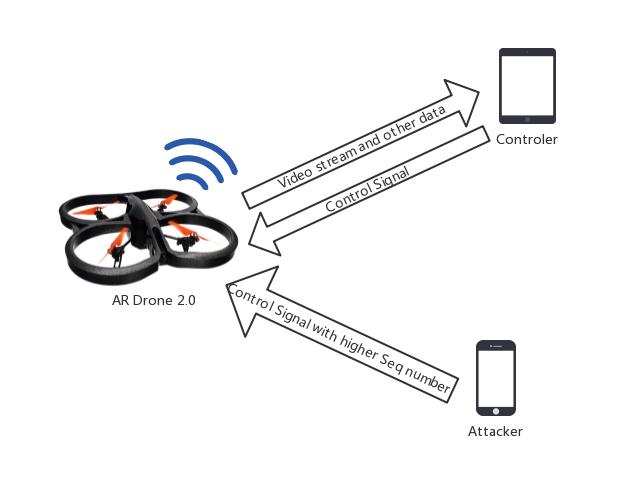
\epsfig{file=figures/Hijack.png, height=1.5in, width=2.5in}
\caption{Hijack Attack Scenario}
\label{hijack}
\end{figure}

The attack consists of the following phases:

\begin{enumerate}
  \item The third-party user uses the Android packet capture application to obtain the target drone IP address,
  \item After the third-party user enters the obtained IP address in this application, he can click the button to send a command to control the drone.
\end{enumerate}


Jpcap provides a class JpcapSender for sending packets, which can be used to send IPPackets and its subclasses, including IPPacket, ICMPPacket, TCPPacket, UDPPacket\cite{jpcap}. After defining a corresponding package, we can use the SendPacket function to send packets. Meanwhile, Jpcap can be used to construct IP data packets to implement sending fake IP.

We try two ways to send UDP packets. A socket can successfully send a UDP packet with the correct source IP address, but an error will occur if the UDP packet sends the source IP address to another host. After reviewing the paper, we found that it was possible to send packets disguised as IP addresses using jpcap, but this approach failed on Android Studio.


\section{Attack on Hubsan H107}

 In this part of our experiment, we use SDR tools to analyze the 2.4GHz radio signal and carry out attack. We found some frequencies used by drone for communication, and recorded these control command signals, which was sent out again by SDR, achieving the effect of interfering with the normal flight of drone.
 

\subsection{Communication Principle}

Communicating via 2.4GHz radio is widely used in many scenes, and controlling is one of them. As shown in figure~\ref{sniff}, we sniffing the radio signal and analyze the frequency used by the drone. The remote control sending instructions via a fixed frequency in a fixed area in 2419MHz - 2466MHz, and the drone receive these instructions. In many types of drones, such as the Hanson H107 Drone we used in our experiment, the message transmit via 2.4GHz radio broadcasts to anyone that can receive it, which means there isn't any connection between remote control and the drone. Not to mention identity verification. Because of the broadcast mechanism and connectionless transmission without identification, this is a primitive way of control, which is easy to attack. The attack model is shown in Figure~\ref{radio}.It is worth noting that after many experiments, we found that after each restart, the communication signal frequency will change in a specific area, there are eight fixed frequency bands. Therefore, we conclude that the drone and remote control first negotiate the frequency band with the drone before sending the flight control command to the remote control, and then only send the flight command to the drone in this frequency band.

\begin{figure}
\centering
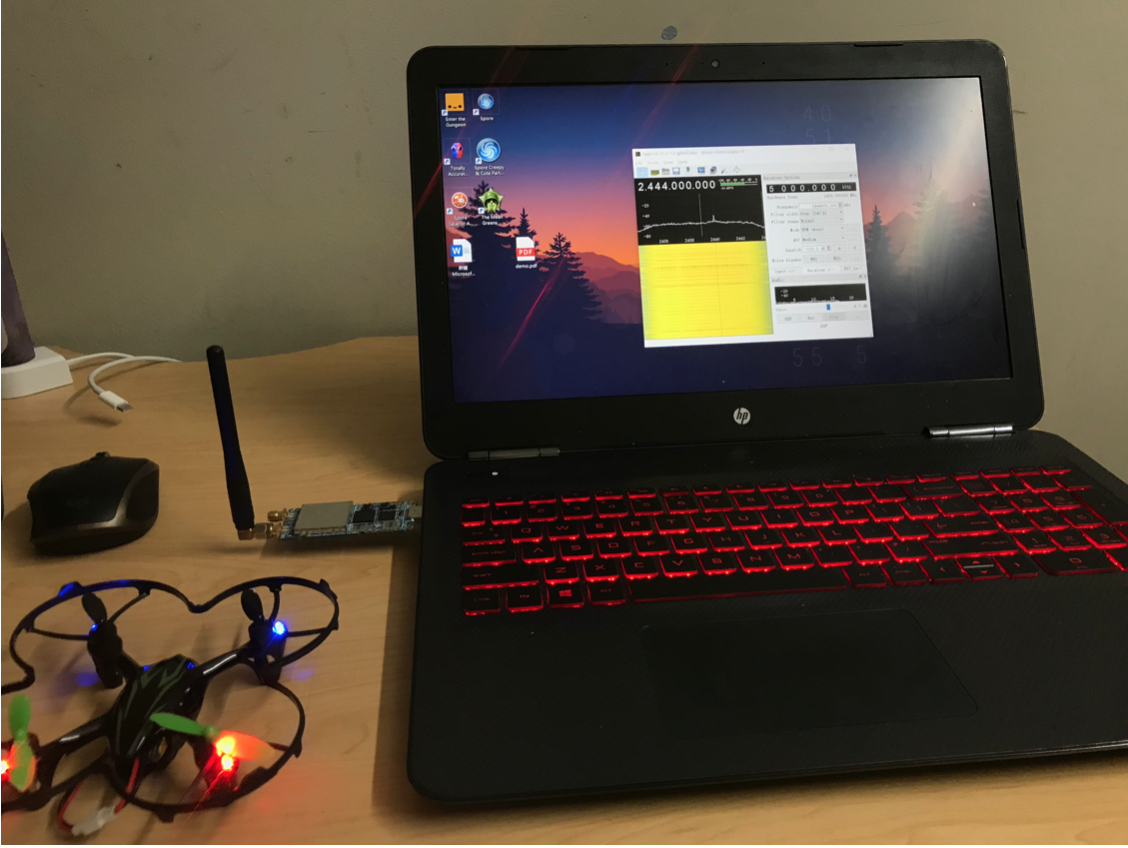
\epsfig{file=figures/sniffTest.png, height=1.3in, width=1.8in}
\caption{Sniffing Test}
\label{sniff}
\end{figure}

\begin{figure}
\centering
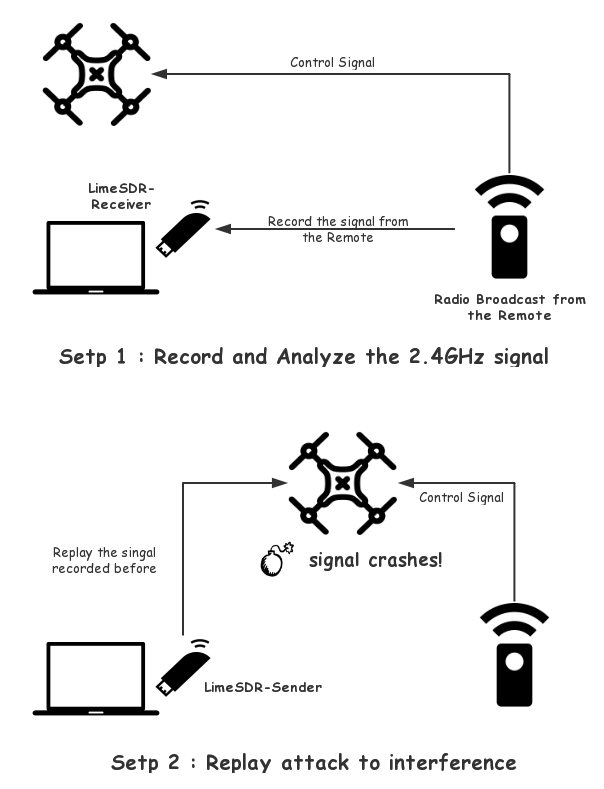
\epsfig{file=figures/radio.png, height=2.5in, width=2in}
\caption{Radio Attack Model}
\label{radio}
\end{figure}

\subsection{Attack}


Since this drone use broadcast to pass signals. There's no connection mechanism between controller and drone and it does not use a mechanism to verify the controller, the attack on this drone is relatively simple. We can use the LimeSDR device to attack the drone. Firstly, we can set up the attack environment on the PC with LimeSDR, gqrx and GNURadio, and then monitor the radio signal in GNURadio. For the reason that the drone and remote control may randomly choose a frequency, to be as easy as possible, we can replay interference signal in all frequency band the drone and the remote control may use. And the running drone can simultaneously monitor the radio signal at 2.4GHz and receive them. Actually, there are two remote controls working at the same time - the real remote control and the LimeSDR, and both of them could be received by the drone. So, our interference signals will effectively affect the normal flight of the aircraft.

\subsection{Result}

Since the drone does not have a mechanism to establish a connection. We can't get his full control, all we can do is interfere with the controller's control, making it insensitive or ineffective. The easiest way is to replay the attack and resend the received signal after a period of time. At this point, the signal from LimeSDR will cause the drone to get out of control or even fall. 

\section{Defense}

The availability of inexpensive drones requires an analysis of potential security and safety threats for such devices. Potential consequences that might be caused by the usage of such drones could be damaging.

\subsection{Securing the AR.DRONE 2.0}

To secure the AR.Drone, an encrypted Wi-Fi connection should be adopted. If the attacker fails to join the network hosted by the drone, attacks mentioned above are impossible.

The approach offered by \cite{hack:secure} is that the drone is just a client and the control device acts as the access point. Users can crosscompile a tool that supports WPA and WPA2 to run on the ARM architecture. Since the drone has a open telnet port with root access, as shown in figure~\ref{telnet}, users can configure the network settings directly. 

\begin{figure}
\centering
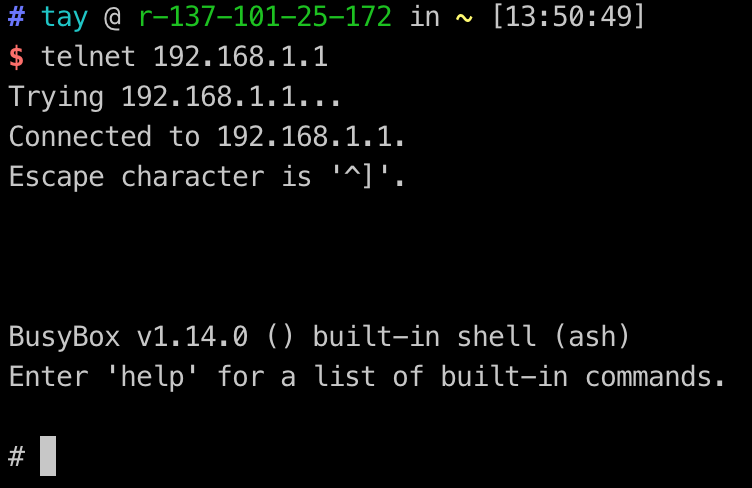
\epsfig{file=figures/telnet.png, height=1.15in, width=2.1in}
\caption{Telnet interface of AR.Drone 2.0}
\label{telnet}
\end{figure}


Given that we have a Wi-Fi Access Point which has authentication manchenism. Its SSID is "SafeAP", the password is "Key2Safe" and its IP address is 192.168.0.1. Fist, let the drone connect to the AP:
\begin{lstlisting}
  iwconfig ath0 mode managed key Key2Safe essid SafeAP
\end{lstlisting}

Then set its ip address as 192.168.0.66 and configure the gateway:

\begin{lstlisting}
ifconfig ath0 192.168.0.66 netmask 255.255.255.0 up
route add default gw 192.168.0.1
\end{lstlisting}

So that anyone who wants to control the drone need to connect to the "SafeAP" first. It protects the vulnerable from vicious connection. This scnario is shown in figure~\ref{client}.

\begin{figure}
\centering
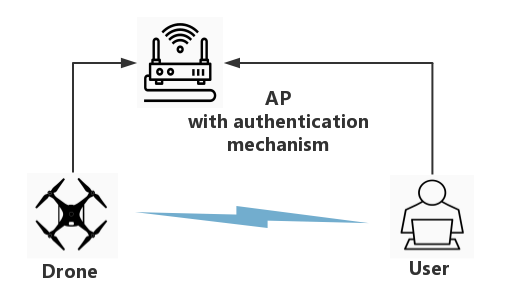
\epsfig{file=figures/droneClient.png, height=1.5in, width=2.4in}
\caption{Drone works in Wi-Fi Infrastructure (Client) mode}
\label{client}
\end{figure}

\subsection{Securing the Hubsan H107}

Because of the simplistic communication mechanism, simply enforcing security is hard to do. To defense against replay attack on Hubsan H107, the developers need to define their own set of security protocols for their own products.
 
 To defend the MITM attacks, there needs to be an authentication mechanism before the remote control can connect to the drone. The drone should ask for an identification from the remote control to establish the connection. So the drone can confirm that the instructions it received came from the correct remote control. And for this authentication mechanism, we can determine the correct remote control by the specific negotiation method. For example, we can determine the remote control through a protocol like the challenge response protocol. As shown in figure~\ref{protocol} :challenge response protocol.The drone and the controller negotiated a password in advance. Firstly, the controller first sends a connection request to the drone. After receiving the connection request, the drone randomly generates a value n and sends the value n to the controller. The controller encode the n by using password. The result c1 will be returned, the drone locally encrypts n with the key to obtain the result c2, and the drone compares c1 and c2. If the two are equal, the controller is an authorized controller. Since n is randomized each time, even if there is a man in the middle, it will not cause any disadvantage to the security of the protocol.

\begin{figure}
\centering
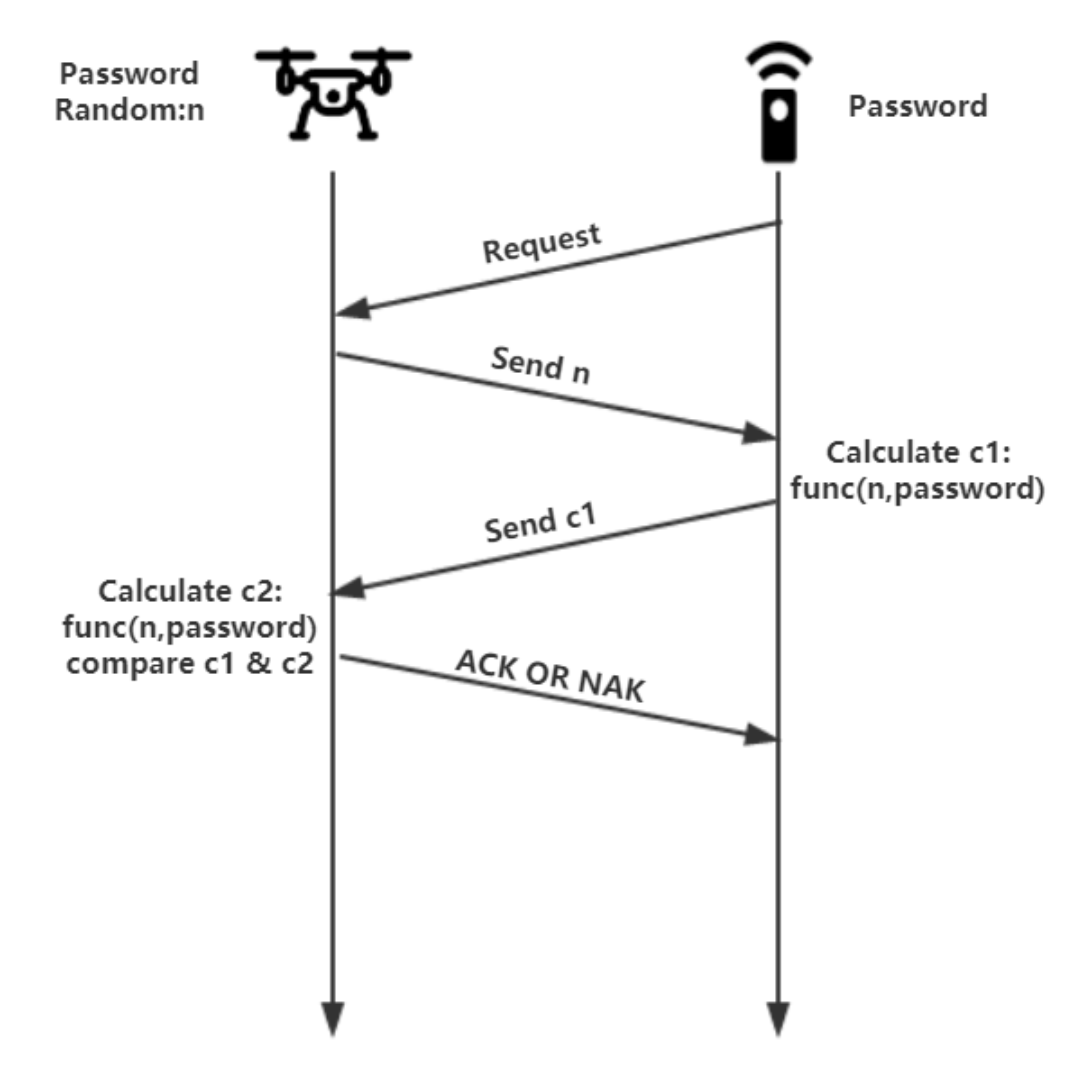
\epsfig{file=figures/protocol.png, height=2in, width=2in}
\caption{Challenge Response Protocol}
\label{protocol}
\end{figure}

To defend the  replay attacks, there should be a sequence number mechanism. The drone will check the serial number of the data it receives. If it receives a command signal with a wrong sequence number, it will ignore this instruction. So that the drone will not be interfered with by the replay attack's instructions.

And we can get some inspiration in the specifications of military radios. In the Hubsan drone, the radio frequency used for communication will be appointed before the remote control begin sending command signal, which is selected from 

about 10 alternative frequencies. It isn't completely fixed, which is good for security, but not enough. The alternative frequencies are too few so that we could conduct our replay attack at every possible frequency, and it works. So, if the drone has a larger number of alternative frequencies, or just use the randomly selected frequency, it will be very hard to attack in this way.

\section{Conclusions}

We have attacked AR.Drone 2.0 and Hubsan H107, using Wi-Fi drone and 2.4GHz radio respectively. 

For the AR.Drone, we can intercept its video signal and seize the control of the drone completely, by sending command messages with a larger sequence number. 

As for the drone controlled by 2.4GHz radio, we have found its communication frequency. We can interfere with the normal flight of the drone by sending command signal which we have recorded. Because of the radio broadcast mechanism, we can't block the original radio signal completely, so we just interfere it.

To prevent the two drones from being attacked, we offered some approaches to securing Wi-Fi and radio connection.

%\end{document}  % This is where a 'short' article might terminate

%ACKNOWLEDGMENTS are optional
\section{Acknowledgments}

We would like to offer our sincere appreciation and thanks to Professor Hugh Anderson for his guidance, enthusiasm and encouragement during the project. He is always generous in providing all kinds of equipment we might need and we are equally grateful to the School of Computing for this. And we also thank our teaching assistant Tan Wang Leng for his insight and expertise. Without them, we wouldn't have gone thus far.


%
% The following two commands are all you need in the
% initial runs of your .tex file to
% produce the bibliography for the citations in your paper.
\bibliographystyle{abbrv}
\bibliography{sigproc}  % sigproc.bib is the name of the Bibliography in this case
% You must have a proper ".bib" file
%  and remember to run:
% latex bibtex latex latex
% to resolve all references
%
% ACM needs 'a single self-contained file'!
%
%APPENDICES are optional
%\balancecolumns

\balancecolumns
% That's all folks!
\end{document}
